%% Template for MLP Coursework 1 / 16 October 2017 

%% Based on  LaTeX template for ICML 2017 - example_paper.tex at 
%%  https://2017.icml.cc/Conferences/2017/StyleAuthorInstructions

\documentclass{article}

\usepackage[T1]{fontenc}
\usepackage{amssymb,amsmath}
\usepackage{txfonts}
\usepackage{microtype}

% For figures
\usepackage{graphicx}
\usepackage{subfigure} 

% For citations
\usepackage{natbib}

% For algorithms
\usepackage{algorithm}
\usepackage{algorithmic}

% the hyperref package is used to produce hyperlinks in the
% resulting PDF.  If this breaks your system, please commend out the
% following usepackage line and replace \usepackage{mlp2017} with
% \usepackage[nohyperref]{mlp2017} below.
\usepackage{hyperref}
\usepackage{url}
\urlstyle{same}

% Packages hyperref and algorithmic misbehave sometimes.  We can fix
% this with the following command.
\newcommand{\theHalgorithm}{\arabic{algorithm}}


% Set up MLP coursework style (based on ICML style)
\usepackage{mlp2017}
\mlptitlerunning{MLP Coursework 1 (\studentNumber)}
\bibliographystyle{icml2017}


\DeclareMathOperator{\softmax}{softmax}
\DeclareMathOperator{\sigmoid}{sigmoid}
\DeclareMathOperator{\sgn}{sgn}
\DeclareMathOperator{\relu}{relu}
\DeclareMathOperator{\lrelu}{lrelu}
\DeclareMathOperator{\elu}{elu}
\DeclareMathOperator{\selu}{selu}
\DeclareMathOperator{\maxout}{maxout}

%% You probably do not need to change anything above this comment

%% REPLACE this with your student number
\def\studentNumber{s1700260}

\begin{document} 

\twocolumn[
\mlptitle{MLP Coursework 1: Activation Functions}

\centerline{\studentNumber}

\vskip 7mm
]

\begin{abstract} 
During recent years, deep neural networks have emerged as one of the most prominent alternatives to solve tasks with machine learning. There are several components and conditions that can modify the behaviour and performance of a deep neural network. In particular, activation functions and parameters initialization methods are of interest to see how a network responds to variations of those components. Different networks with distinct numbers of layers can solve the same task but their performance can be different as well. In this report, I present the results and provide a discussion of experiments to compare the performance of deep neural networks by varying the activation functions, the parameters initialization approaches and the number of hidden layers.
\end{abstract} 

\section{Introduction}
\label{sec:intro}
In machine learning, a given task can be solved using a variety of algorithms; each of those algorithms has its own behaviour and performance. Moreover, the behaviour and results thrown by a certain model can vary depending on a multitude of aspects, including the initial conditions and the definition of its components and hyperparameters. This document presents a report of experiments ran over a set of deep neural networks. The main objective is to compare the results and behaviours of the models and provide discussion about them.

The experiments were ran using the \href{http://yann.lecun.com/exdb/mnist/}{MNIST} database of handwritten digit images. This database contains grayscale examples of handwritten digits from 0 to 9. Each example has 784 features which correspond to the number of pixels (28 x 28). The database has a training set of 60000 examples and a test set of 10000 examples. Just the training set was used in the experiments; it was split into two parts. The first part with 50000 examples was used for the training stage; the second part containing 10000 examples was used for validation.

Three kinds of experiments were performed. The first one was aimed to compare the behaviour of different types of activations, in particular, variants of the Restricted Linear Unit (ReLU) ~\citep{act_relu}. The second type of experiments was focused on the impact of the depth of a network with respect to accuracy. Finally, the last sort of experiments was addressed to investigate the results of different approaches of weight initialization.


\section{Activation functions}
\label{sec:actfn}
In neural networks, activation functions are meant to indicate if a neuron should be activated or not. In classification tasks, one of the most common activations is the Sigmoid function (equation 1). However, the problem with this activation is the small values of its gradient (equation 2) for high input values (which reduces the process of learning).

\begin{equation}
  \sigmoid(x) = \frac{1}{1 + e^{-x}}
\end{equation} 

\begin{equation}
  \frac{d}{dx} \sigmoid(x) = \sigmoid(x)(1 - \sigmoid(x))
\end{equation} 


Several functions have emerged to solve the problem of sigmoid. One of them is ReLU (equation 3), which has a constant gradient (equation 4) that results in faster learning.

\begin{equation}
  \relu(x) =
     \begin{cases} 
      0      & \quad \text{if } x \leq  0 \\
      x       & \quad \text{if } x > 0 .
    \end{cases} 
\end{equation}

\begin{equation}
  \frac{d}{dx} \relu(x) =
     \begin{cases} 
      0      & \quad \text{if } x \leq  0 \\
      1       & \quad \text{if } x > 0 .
    \end{cases} 
\end{equation}

Even though ReLU solves the slow learning problem related to Sigmoid, it has some issues as well. In the region where ReLU is a horizontal line, the gradient is 0, which means that the weights are not updated during gradient descent. This means that the neurons in that situation will not respond to variations in error and 'will die'. The alternative to avoid that problem is to provide a gradient different to 0 over the entire space of the activation function. The first approach to accomplish that goal is the Leaky ReLU function (equation 5) ~\citep{act_lrelu} which is a slight variation of ReLU that provides a small gradient (equation 6) for negative input values. For the experiments of this report, \(\alpha\) = 0.01

\begin{equation}
  \lrelu(x) =
     \begin{cases} 
      \alpha x      & \quad \text{if } x \leq  0 \\
      x       & \quad \text{if } x > 0 .
    \end{cases} 
\end{equation}

\begin{equation}
  \frac{d}{dx} \lrelu(x) =
     \begin{cases} 
      \alpha      & \quad \text{if } x \leq  0 \\
      1       & \quad \text{if } x > 0 .
    \end{cases} 
\end{equation}

There are other alternatives to ReLU, one of them is the Exponential Linear Unit function (ELU) (equation 7) ~\citep{act_elu}. One of the main objectives of this activation function is to get a gradient (equation 8) that is closer to a natural gradient, something that does not happen with Leaky ReLu since there is an abrupt change in the gradient at point 0 (where the slope of the function changes.) For the experiments of this report, \(\alpha\) = 1

\begin{equation}
  \elu(x) =
     \begin{cases} 
      \alpha (e^{x} - 1)     & \quad \text{if } x \leq  0 \\
      x       & \quad \text{if } x > 0 .
    \end{cases} 
\end{equation}

\begin{equation}
  \frac{d}{dx} \elu(x) =
     \begin{cases} 
      \elu(x) + \alpha      & \quad \text{if } x \leq  0 \\
      1       & \quad \text{if } x > 0 .
    \end{cases} 
\end{equation}

Finally, Scaled Exponential Linear Unit function (SELU) (equation 9) ~\citep{act_selu} is an activated function which is the heart of Self Normalizing Networks (SNN). As stated in its name, this kind of networks are meant to have layers that output normalized values; this is in part accomplished by using SELU activations. The derivative of this activation is similar to ELU's one (equation 10). For scaled inputs (\(\mu\) = 0, \(\sigma\) = 1), the values for \(\alpha\) and \(\gamma\) are 1.6733 and 1.0507 respectively.

\begin{equation}
  \selu(x) = \lambda
     \begin{cases} 
      \alpha (e^{x} - 1)     & \quad \text{if } x \leq  0 \\
      x       & \quad \text{if } x > 0 .
    \end{cases} 
\end{equation}

\begin{equation}
  \frac{d}{dx} \selu(x) =
     \begin{cases} 
      \selu(x) + \lambda\alpha      & \quad \text{if } x \leq  0 \\
      \lambda       & \quad \text{if } x > 0 .
    \end{cases} 
\end{equation}

\section{Initialization approaches}
\label{sec:actexpts}
The ultimate goal of a neural network is to find values for its parameters to allow making accurate predictions. Originally, there is no reason to set the parameters with certain values, however, in terms of efficient backpropagation ~\citep{init_lecun}, when using sigmoid activations the recommendation is to set the weights in a way that the activation is primarily activated in its linear region. 

One of the options to do that is to set the weights randomly from a uniform distribution $U(low, high)\) with zero mean. From that point, the first alternative corresponds to constraining the estimated variance of a unit to be independent of the number of incoming connections $w_i \sim U(-\sqrt{3/n_{in}}, \sqrt{3/n_{in}}$); the second option constrains the estimated variance of a unit's gradient to be independent of the number of outgoing connections $w_i \sim U(-\sqrt{3/n_{out}}, \sqrt{3/n_{out}}$), and the last one is the Glorot and Bengio's combined initialization $w_i \sim U \left(-\sqrt{6/(n_{in}+n_{out})}, \sqrt{6/(n_{in}+n_{out})}\right)$) ~\citep{init_glorot}

An additional initialization strategy corresponds to the one used by SNNs which uses a normal distribution with \(\mu\) = 0, \(\sigma\) = $1/n_{out}$  which along with SELU activations are the core of that kind of networks.

\section{Experimental comparison of activation functions}
\label{sec:actexpts}
In this stage, I used a neural network with 2 hidden layers (with their corresponding activations) with 100 hidden units per layer. The error was calculated using the Cross Entropy of the Softmax function (equation 11) which has a derivative defined in equation 12 . The models were trained for a total of 100 epochs with a batch size of 100. Four learning rates were used for every experiment (0.001, 0.01, 0.05, 0.1). The baseline systems for comparison used Sigmoid and ReLU activations.
\begin{equation}
	E^{(b)} = -\sum_{d=1}^D \lbrace t^{(b)}_d \log\left[\textrm{Softmax}_d\left({y}^{(b)}\right)\right]\rbrace
\end{equation}
\begin{equation}
     \frac{dE^{(b)}}{dy^{(b)}_d} = \textrm{Softmax}_d \left({y}^{(b)}\right) - t_d
\end{equation}


As depicted in Figure 1, it is clearly evident that the validation error has a similar evolution for ReLU and its variant activations; they even tend to converge for small learning rate values. However, as the learning rate increases, the convergence is less evident and the difference between them increases. Also after several numbers of epochs, their validation errors start to grow with a similar rate which suggests that none of them is more robust to overfitting than the others. It is also worth to note that ReLU and its variant activations have faster speed rates than Sigmoid; nonetheless, for higher learning rates the later is more stable and more robust to overfitting.

Finally,  Figure 2 shows the training time for each activation with every learning rate. There is a clear pattern where the variants of ReLU have higher training times than ReLU itself, being ELU and SELU the ones with more relevant and similar difference, which is expected since they implement more complex functions.


\begin{figure}[tb]
\vskip 5mm
\begin{center}
\centerline{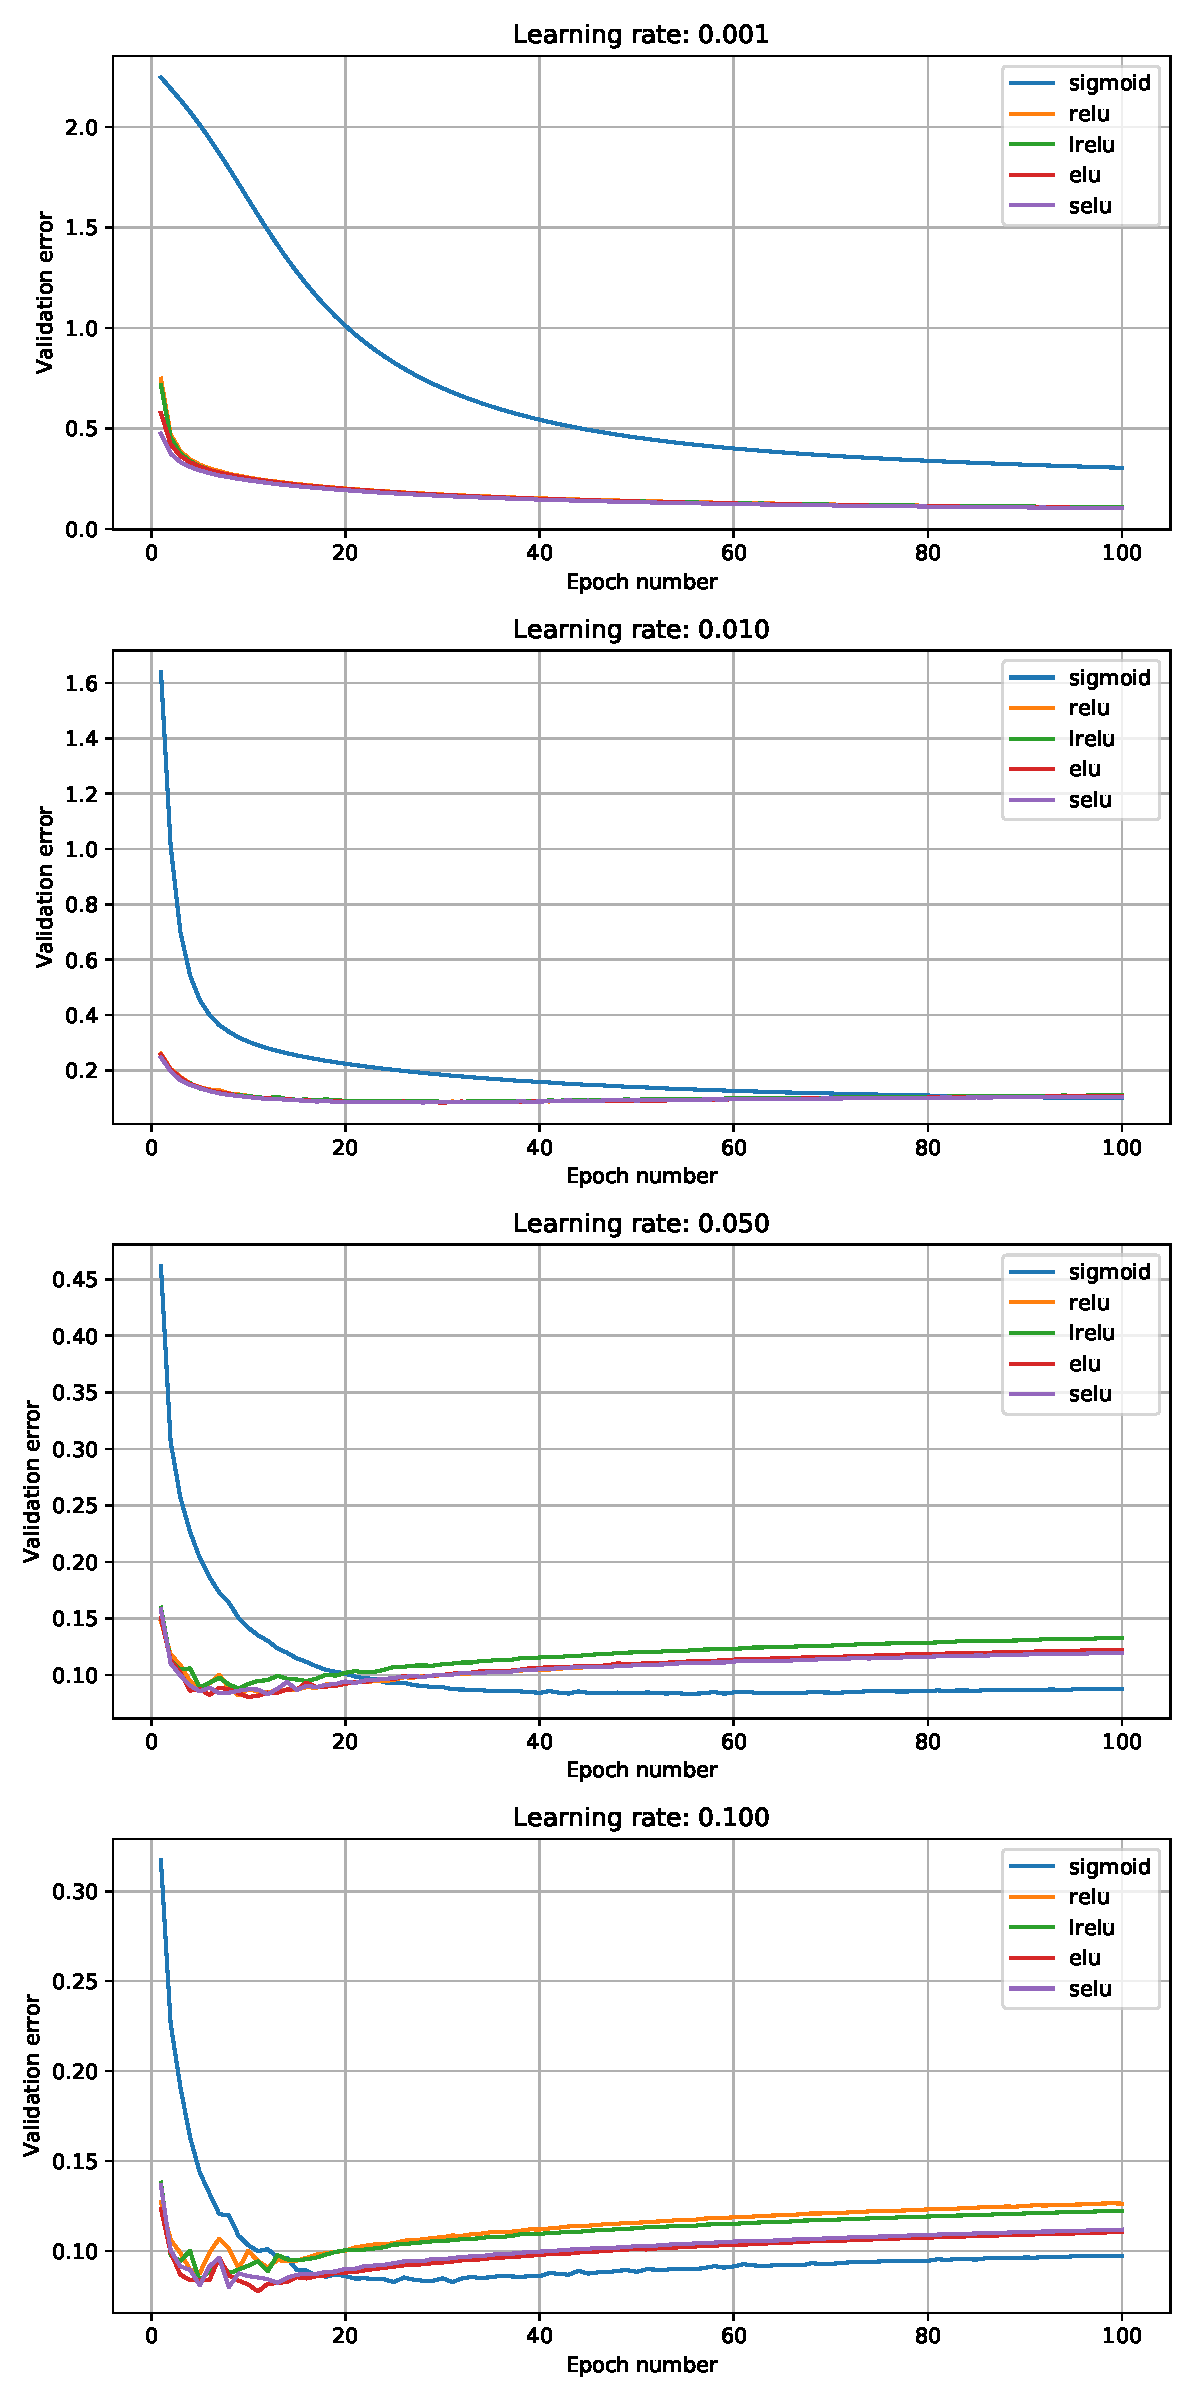
\includegraphics[width=60mm]{activations_val_error}}
\caption{Validation error for different kinds of activations}
\label{fig:activations_val_error}
\end{center}
\vskip -5mm
\end{figure} 

\begin{figure}[tb]
\vskip 5mm
\begin{center}
\centerline{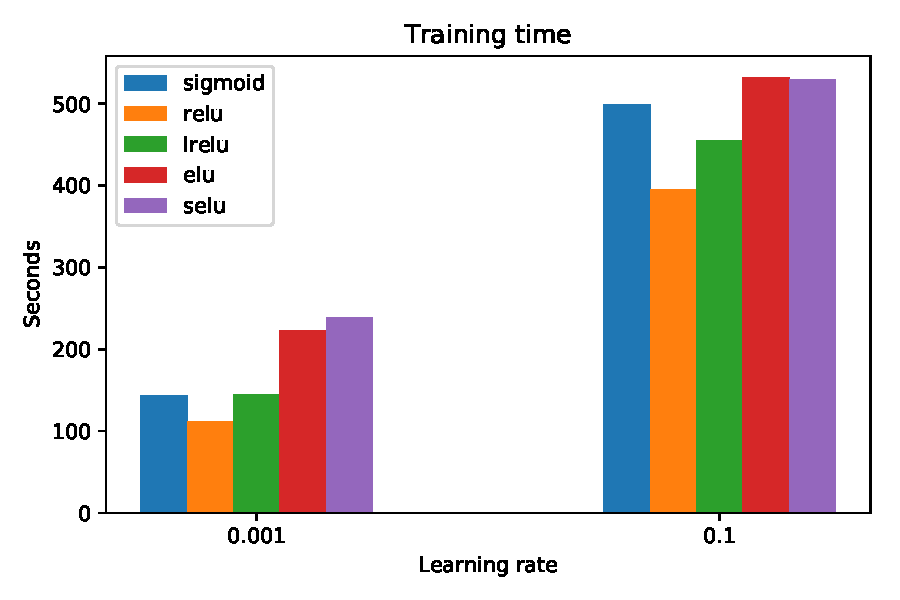
\includegraphics[width=50mm]{activations_training_time}}
\caption{Training time for different kinds of activations}
\label{fig:activations_training_time}
\end{center}
\vskip -5mm
\end{figure} 

\section{Deep neural network experiments}
\label{sec:dnnexpts}

\subsection{Number of layers}

In this section, I used a set of neural networks with 2 to 8 hidden layers using SELU activations for each of them. Similarly to the previous stage, every hidden layer was set with 100 hidden units; the models were trained for a total of 100 epochs with a batch size of 100; the learning rate was 0.001. 

Figure 3 shows the evolution of the validation accuracy and error for every network. It is evident that the higher the number of layers, the faster the accuracy increases. However, the training time increases along with the number of layers as seen in Figure 4. Moreover, with more than 4 layers there is no much gain in how fast the accuracy increases, and in the last epochs, there is no much difference in the accuracy of all networks.

\begin{figure}[tb]
\vskip 5mm
\begin{center}
\centerline{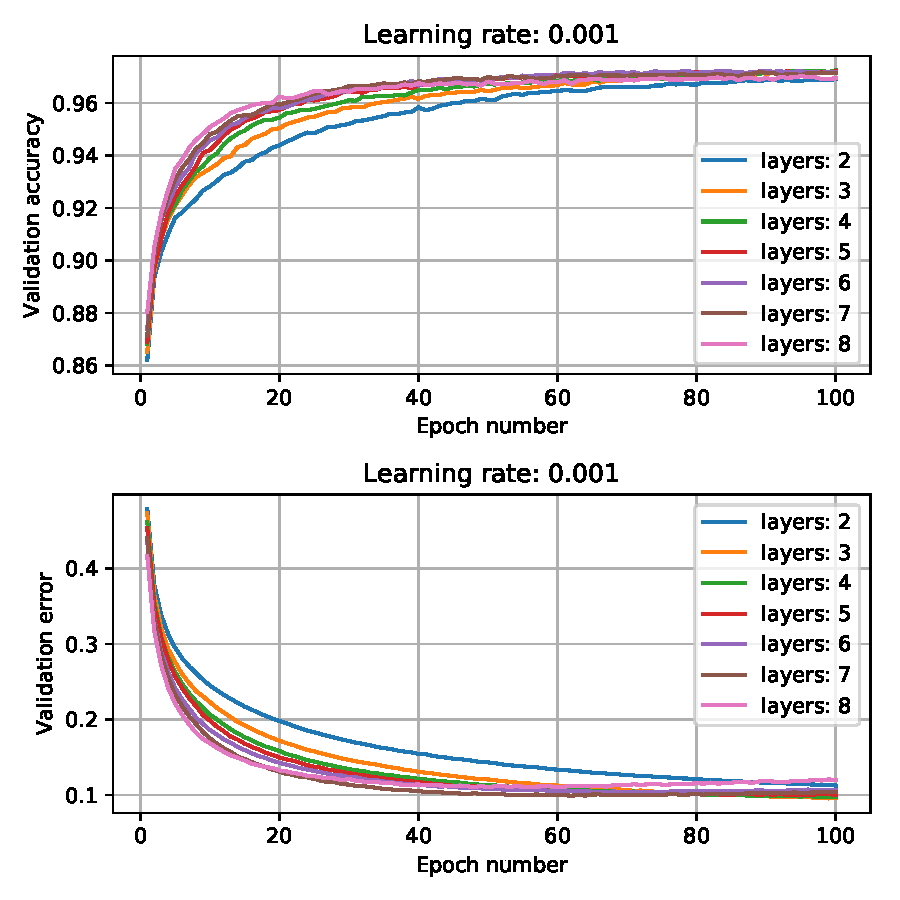
\includegraphics[width=60mm]{validation_acc_err_mult_layers}}
\caption{Validation accuracy and error for networks with different number of hidden layers}
\label{fig:validation_acc_err_mult_layers}
\end{center}
\vskip -5mm
\end{figure} 

\begin{figure}[tb]
\vskip 5mm
\begin{center}
\centerline{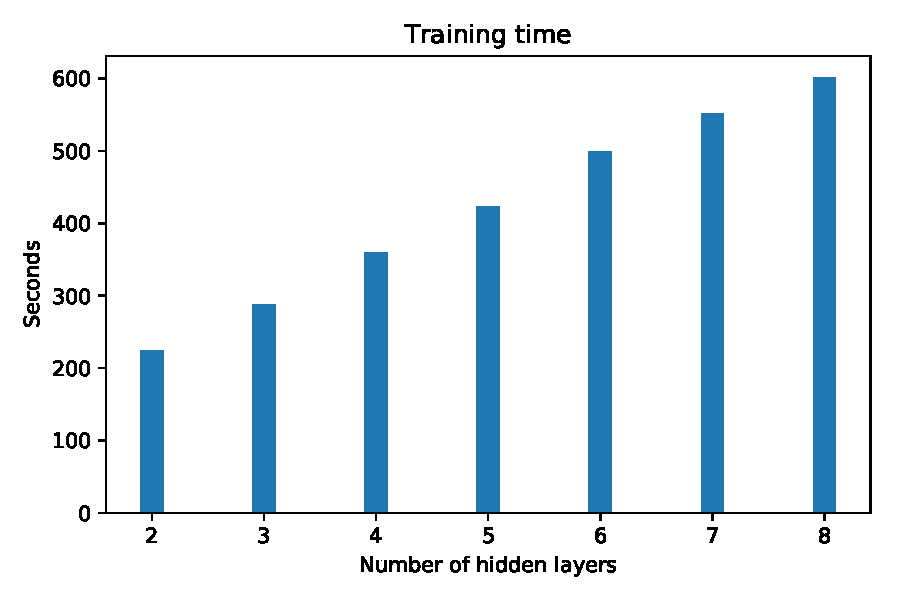
\includegraphics[width=50mm]{training_time_mult_layers}}
\caption{Training time for networks with different number of hidden layers}
\label{fig:training_time_mult_layers}
\end{center}
\vskip -5mm
\end{figure} 

In addition, after a number of epochs, the validation error of the network with a higher number of layers tend to increase which means that the models start to overfit. This is an expected result since the higher the complexity of a model, the higher the chances to overfit. This particular experiment is a clear example of the Occam's razor, where the simpler networks are better.

\subsection{ Different Initialisation approaches}

In this part, I used a neural network with 2 hidden layers; every hidden layer was set with 100 hidden units; the model was trained for a total of 100 epochs with a batch size of 100; the learning rate was 0.001. I used the initialization strategies defined in section 3 of this report. 

Figure 5 shows how the network behaves quite different for SELU initialization, even though the learning process is slower, it also converges with the other initialisation options. Moreover, due to the rate of reduction in validation error, it seems that there is a room for improving the results with more epochs.

\begin{figure}[tb]
\vskip 5mm
\begin{center}
\centerline{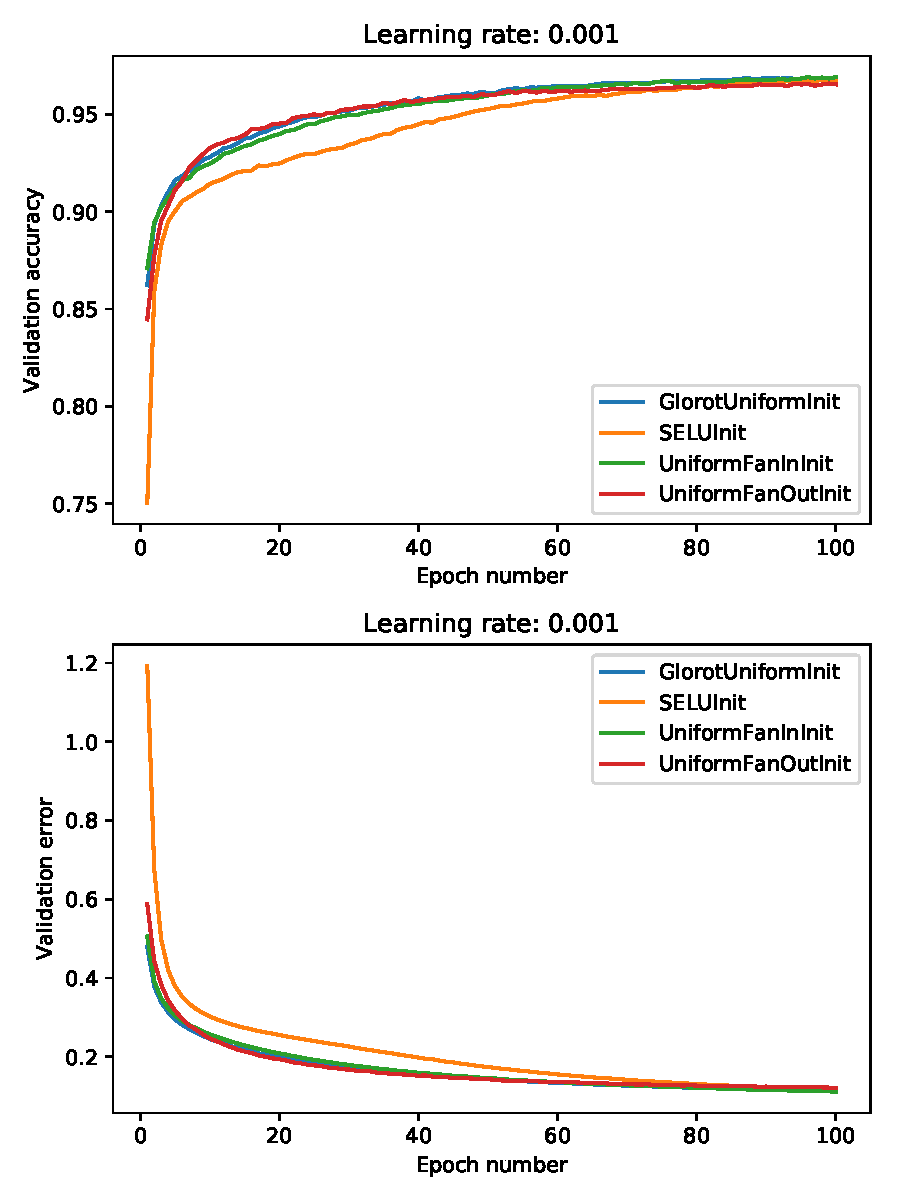
\includegraphics[width=60mm]{validation_acc_err_init}}
\caption{Validation accuracy and error for different types of initialization strategies}
\label{fig:validation_acc_err_init}
\end{center}
\vskip -5mm
\end{figure}


\section{Conclusions}
\label{sec:concl}
As mentioned previously, there are several aspects that influence the results of a machine learning algorithm. Particularly, in neural networks, the activation functions play an important role on how a network behaves. That was clearly evident in the experiments described in this report, where different activation functions lead to different results; especially when the functions are quite different. Also, the complexity of a neural network has an impact on the results, however, as seen in the experiments, a more complex network does not necessarily make a better job. Finally, the experiments also showed that the way how the parameters of a network are initialized influences its behaviour as well.

The experiments detailed in this report were performed over a well-known task. Further experiments should be aimed to measure the impact in the results in other kinds of tasks like regression or transcription

\bibliography{cw1-refs}
\bibliographystyle{plainnat}

\end{document} 


% This document was modified from the file originally made available by
% Pat Langley and Andrea Danyluk for ICML-2K. This version was
% created by Lise Getoor and Tobias Scheffer, it was slightly modified  
% from the 2010 version by Thorsten Joachims & Johannes Fuernkranz, 
% slightly modified from the 2009 version by Kiri Wagstaff and 
% Sam Roweis's 2008 version, which is slightly modified from 
% Prasad Tadepalli's 2007 version which is a lightly 
% changed version of the previous year's version by Andrew Moore, 
% which was in turn edited from those of Kristian Kersting and 
% Codrina Lauth. Alex Smola contributed to the algorithmic style files.  
